\documentclass[11pt,letterpaper]{article}
% ---------------------------------------------------------------------------
% Preámbulo compartido (v2): tipografía, color, cuadros, figuras y cabeceras.
% Compilar con XeLaTeX. Todo lo que depende de papers.json llega por
% build/metadata.tex como macros semánticas (\papertitle, \paperauthors, ...).
% ---------------------------------------------------------------------------
\usepackage{fontspec}
% Serifa para el cuerpo: TeX Gyre Pagella (incluida en TeX Live completo).
\setmainfont{texgyrepagella}[Extension=.otf,UprightFont=*-regular,BoldFont=*-bold,
  ItalicFont=*-italic,BoldItalicFont=*-bolditalic,Scale=0.95]
% Sans para títulos, cuadros y figuras: TeX Gyre Heros.
\setsansfont{texgyreheros}[Extension=.otf,UprightFont=*-regular,BoldFont=*-bold,
  ItalicFont=*-italic,BoldItalicFont=*-bolditalic,Scale=MatchLowercase]
\setmonofont{Latin Modern Mono}[Scale=0.85]
\usepackage{polyglossia}
\setdefaultlanguage{spanish}
\setotherlanguage{english}
\usepackage[letterpaper,margin=27mm,headsep=7mm,footskip=11mm]{geometry}
\usepackage{microtype,graphicx,amsmath}
\usepackage{xcolor,placeins,etoolbox}
\usepackage{booktabs,tabularx,threeparttable,ragged2e}
\usepackage{enumitem}
\usepackage{titlesec}
\usepackage{caption}
\usepackage{fancyhdr}
\usepackage[hidelinks,unicode]{hyperref}
\usepackage{xurl}
\usepackage[autostyle]{csquotes}

% --- Paleta: un acento y un gris. Los cuadros permanecen en negro. -----------
\definecolor{tinta}{RGB}{23,59,54}    % acento (títulos, rótulos, trazos)
\definecolor{gris}{RGB}{107,107,102}  % cabeceras y notas discretas
\definecolor{humo}{RGB}{213,221,212}  % filetes muy suaves (solo figuras)

% --- Párrafo y página ----------------------------------------------------------
\linespread{1.04}
\setlength{\parskip}{0.3em}
\setlength{\parindent}{1.1em}
\setlength{\emergencystretch}{3em}
\tolerance=600 \hbadness=10000
\widowpenalty=10000 \clubpenalty=10000
\setlist{nosep}
\setcounter{secnumdepth}{3}

% --- Títulos de sección: sans, acento, numeración con punto (nivel 1) ---------
\titleformat{\section}{\sffamily\bfseries\large\color{tinta}}{\thesection.}{0.6em}{}
\titlespacing*{\section}{0pt}{1.6em}{0.6em}
\titleformat{\subsection}{\sffamily\bfseries\normalsize}{\thesubsection}{0.6em}{}
\titlespacing*{\subsection}{0pt}{1.1em}{0.35em}
\titleformat{\subsubsection}{\sffamily\itshape\normalsize}{\thesubsubsection}{0.6em}{}
\titleformat{\paragraph}[runin]{\itshape}{}{0pt}{}[.]

% --- Leyendas: rótulo en sans y acento, texto pequeño, alineado a la izquierda --
\captionsetup{font=small,labelfont={sf,bf,color=tinta},labelsep=period,
  justification=raggedright,singlelinecheck=false,skip=5pt}
\captionsetup[table]{position=above,skip=3pt}
\captionsetup[figure]{position=below}

% --- Cuadros: sans pequeña, sin líneas internas ni sombreado (guía del Boletín)
% Los flotantes reinician la fuente; el gancho correcto es \@floatboxreset.
\makeatletter
\g@addto@macro\@floatboxreset{\centering\ifdefstring{\@captype}{table}{\sffamily\small}{}}
\makeatother
\renewcommand{\arraystretch}{1.15}
\setlength{\tabcolsep}{5pt}
\setlength{\aboverulesep}{0.45ex}
\setlength{\belowrulesep}{0.65ex}
\newcolumntype{Y}{>{\RaggedRight\arraybackslash}X}  % texto, sin justificar
\newcolumntype{Z}{>{\RaggedLeft\arraybackslash}X}   % cifras alineadas a la derecha
\newcommand{\nd}{---}                               % dato no documentado
\newcommand{\aprox}{\ensuremath{\approx}}
\newcommand{\mayor}{\ensuremath{>}}
\newcommand{\menor}{\ensuremath{<}}
\newcommand{\cabecera}[1]{\textbf{#1}}              % cabecera de columna
\newcommand{\fila}[1]{\textbf{#1}}                  % rótulo de fila
% Notas al pie de cuadro: \begin{tablenotes}[flushleft]\footnotesize ... \end{tablenotes}
\appto\TPTnoteSettings{\footnotesize\color{gris}\RaggedRight}

% --- Cabecera y pie ------------------------------------------------------------
\pagestyle{fancy}\fancyhf{}
\renewcommand{\headrulewidth}{0pt}
\setlength{\headheight}{14pt}
\fancyhead[L]{\footnotesize\sffamily\color{gris}\papershorttitle}
\fancyhead[R]{\footnotesize\sffamily\color{gris}%
  \ifdefstring{\paperstatus}{draft}{Borrador \textperiodcentered{} fuentes: \sourcerevision}{}}
\fancyfoot[C]{\small\sffamily\thepage}
\fancypagestyle{plain}{\fancyhf{}\renewcommand{\headrulewidth}{0pt}%
  \fancyfoot[C]{\small\sffamily\thepage}%
  \fancyhead[R]{\footnotesize\sffamily\color{gris}%
    \ifdefstring{\paperstatus}{draft}{Borrador \textperiodcentered{} fuentes: \sourcerevision}{}}}

% --- Bloque de título (datos desde build/metadata.tex) -------------------------
\newcommand{\paperheading}{%
  \thispagestyle{plain}%
  \begin{center}
    {\sffamily\bfseries\Large\color{tinta}\papertitle\par}\vspace{0.55em}
    {\itshape\papertitleen\par}\vspace{1.2em}
    {\paperauthors\par}\vspace{0.45em}
    {\small\paperaffiliations\par}\vspace{0.25em}
    {\small\color{gris}Correspondencia: \papercontact\par}
  \end{center}
  \vspace{0.3em}{\color{tinta}\hrule height 0.5pt}\vspace{1.1em}}

% --- Resúmenes y palabras clave: medida algo más estrecha, rótulo en acento ---
\newenvironment{bloqueresumen}[1]{%
  \par\begingroup\small
  \setlength{\leftskip}{7mm}\setlength{\rightskip}{7mm}\setlength{\parindent}{0pt}
  \noindent{\sffamily\bfseries\color{tinta}#1.}\enspace\ignorespaces}{\par\endgroup}
\newcommand{\clave}[2]{\par\begingroup\small
  \setlength{\leftskip}{7mm}\setlength{\rightskip}{7mm}\setlength{\parindent}{0pt}
  \noindent{\sffamily\bfseries\color{tinta}#1:}\enspace #2\par\endgroup\medskip}

% --- Compatibilidad con el verificador: el banner ya no se invoca en el cuerpo --
\newcommand{\draftnotice}{}
\newcommand{\editorialtodo}[1]{\textbf{[Revisión editorial: #1]}}

\input{build/metadata}
\begin{document}
\paperheading
\begin{bloqueresumen}{Resumen}La diversidad de equipos y configuraciones puede desplazar tiempo de formación científica hacia la resolución de problemas de instalación. Se describe una arquitectura de entornos de trabajo reproducibles basada en repositorios Git, contenedores de desarrollo, cuadernos y automatización, contextualizada en SILAFAE XV y la CERN School of Computing de América Latina de 2026. El enfoque conecta preparación del entorno, ejecución del análisis y conservación de resultados. Se presenta la observación comunicada por el autor de una preparación para 80 estudiantes en menos de diez minutos, indicando que su interpretación requiere precisar el intervalo y recuperar registros operativos. Se distingue esa observación de una evaluación controlada del aprendizaje. Como demostrador complementario, los propios manuscritos se gestionan en LaTeX y generan PDF mediante integración continua. Se discuten conectividad, cuotas, mantenimiento, portabilidad y una propuesta de evaluación reproducible para futuras escuelas.
\end{bloqueresumen}
\clave{Palabras clave}{computación científica; física; reproducibilidad; Git; automatización; formación.}
\begin{english}
\begin{bloqueresumen}{Abstract}Practical physics education requires environments that support analysis, review of decisions, and preservation of results. This technical essay presents an architecture based on Git, development containers, notebooks, and automation. Documentary analysis compares Codespaces, Binder, JupyterHub, and Colab in terms of administration, persistence, and operational constraints, contextualized in Latin American teaching materials. Results distinguish repository availability, verifiable execution, and session evaluation as separate objects. A proposed protocol separates instructor preparation, student onboarding, resource consumption, and scientific interpretation, supported by recording templates. The analysis explains how infrastructure can be selected according to the task and available support, and how reproducible practices can transfer to other activities. The editorial repository provides an executable example of the same procedure.
\end{bloqueresumen}
\clave{Keywords}{scientific computing; physics; reproducibility; Git; automation; education.}
\end{english}
\section{Introducción}
En una sesión práctica de física, el tiempo disponible debe permitir formular preguntas, ejecutar análisis e interpretar resultados. Sin embargo, la diversidad de sistemas operativos, bibliotecas y permisos puede convertir el inicio de la clase en una serie de instalaciones individuales. El problema no se limita a comodidad técnica: si cada estudiante parte de un entorno distinto, resulta más difícil distinguir un error conceptual de uno causado por la configuración.

Las buenas prácticas de computación científica relacionan organización de archivos, control de versiones y automatización con la posibilidad de comprender y repetir el trabajo \cite{wilson}. Incorporarlas a la formación permite que el estudiante aprenda tanto el contenido de un análisis como las condiciones que lo hacen verificable. No se trata de ocultar la infraestructura indefinidamente, sino de decidir qué complejidad abordar en cada momento de una secuencia docente.

En América Latina, las propuestas de computación transversal han planteado compartir protocolos, servicios y capacidades entre proyectos e instituciones \cite{transversal,whitepaper}. El término transversal se utiliza aquí para describir prácticas reutilizables más allá de un experimento: organizar código y datos, definir dependencias, ejecutar tareas, registrar resultados y comunicar cambios. La formación en física ofrece un contexto concreto para aprenderlas, mientras su utilidad puede extenderse a otras áreas científicas.

Este trabajo desarrolla el resumen aceptado como contribución 667 de ICHEP 2026 \cite{abstract}. Describe una arquitectura docente, sitúa su aplicación en SILAFAE XV y CSC América Latina 2026, y propone cómo evaluar sus resultados sin confundir rapidez de preparación con aprendizaje. Añade un demostrador editorial: los artículos de este proyecto se compilan mediante un flujo que conserva las fuentes y actualiza los PDF en el mismo repositorio. El alcance es un informe técnico y una propuesta metodológica; no se presenta un ensayo educativo controlado.

\section{Antecedentes: acceso, infraestructura y continuidad}
La experiencia venezolana con ATLAS Open Data muestra que los datos abiertos pueden utilizarse en trabajos de pregrado y posgrado con herramientas de análisis y acompañamiento académico \cite{atlas}. La existencia de un conjunto de datos es una condición de partida; una actividad formativa necesita además ejemplos ejecutables, documentación y una pregunta adecuada a su duración. La accesibilidad debe evaluarse en esa combinación.

Los materiales de contexto aportados por el autor identifican dos antecedentes técnicos: la contribución CHEP 2018 sobre Open Key y el despliegue multiusuario propuesto en CHEP 2021 \cite{contexto,chep}. Su relación con el presente trabajo es la búsqueda de un punto de partida utilizable para estudiantes. Un entorno transportable, un servicio compartido y un espacio en la nube resuelven problemas parcialmente distintos. No se plantea una sustitución universal de los recursos locales por servicios externos.

El documento de estrategia de 2024 propone aprovechar recursos y capacidades compartidos para investigación y formación \cite{whitepaper}. El presente manuscrito se concentra en una escala operativa: un repositorio de ejercicios, un entorno descrito explícitamente y una secuencia de análisis. La contribución consiste en relacionar esas piezas con el proceso docente y con un protocolo de verificación. La portabilidad se considera una propiedad que debe probarse, no una consecuencia automática de usar Git.

\subsection{De ROOT en la web a la formación comunitaria en software}
Una presentación de Sánchez Pineda en el ROOT Workshop de septiembre de 2015 ya relacionaba interfaces web para analizar datos de ATLAS con tutoriales de ROOT y actividades de CEVALE2VE \cite{root2015}. Este antecedente sitúa el acceso mediante navegador dentro de una trayectoria anterior a Codespaces. Las herramientas y los despliegues han cambiado, pero permanece una pregunta docente: cómo acercar el análisis de física a estudiantes con recursos y experiencia heterogéneos.

El artículo colectivo \emph{Software Training in HEP}, del que Sánchez Pineda es coautor, organiza la formación en competencias generales de software, herramientas específicas de física y técnicas avanzadas \cite{hsftraining}. Esa distinción permite situar Git y la integración continua como competencias transferibles, junto con herramientas disciplinares como ROOT. El presente trabajo desarrolla una aplicación docente de esa combinación; no propone que el uso de una plataforma concreta constituya por sí mismo una competencia científica.

\subsection{ESCAPE y los entornos virtuales de investigación}
ESCAPE vincula infraestructuras de física de partículas y astrofísica con servicios de ciencia abierta \cite{escape}. Su directorio de herramientas reúne accesos a JupyterHub, entornos Docker, documentación de Rucio, repositorios de software, tutoriales y recursos de ATLAS Open Data \cite{escapetools}. El Virtual Research Environment documentado por VRE Hub busca facilitar flujos de análisis completos y la preservación de resultados conforme a principios FAIR \cite{vrehub}.

Estas fuentes permiten comparar dos escalas de trabajo. Un entorno virtual de investigación articula servicios y recursos de una infraestructura compartida; el repositorio docente aquí descrito delimita un ejercicio y sus dependencias para una sesión de formación. Comparten la necesidad de documentar el entorno, pero no son sistemas equivalentes. No se atribuye a los talleres de este estudio el uso de los servicios de ESCAPE sin registros que lo documenten. La contribución de esta comparación es identificar requisitos reutilizables: acceso a datos, descripción del software y conservación del procedimiento.

\section{Arquitectura del entorno docente}
\subsection{Separar contenido, entorno y ejecución}
La arquitectura distingue tres capas. La primera contiene el problema científico: datos de ejemplo, ejercicios, explicaciones y criterios de interpretación. La segunda define el software necesario para trabajar. La tercera ejecuta comprobaciones y produce salidas. Esta separación permite modificar una pregunta sin rediseñar el entorno, o actualizar una dependencia sin reescribir toda la actividad.

Los contenedores de desarrollo describen un entorno mediante archivos versionados; GitHub Codespaces puede utilizarlos para ofrecer un espacio accesible desde el navegador \cite{devcontainers}. Esta descripción debe incluir dependencias y comandos de preparación. El acceso web reduce la necesidad de instalar herramientas científicas en cada equipo, pero sigue requiriendo una cuenta, conectividad y recursos disponibles. Un entorno descrito no es necesariamente inmutable: imágenes etiquetadas y paquetes sin fijar pueden cambiar entre ejecuciones.

Los repositorios docentes citados en el resumen incluyen \texttt{jupyter-on-codespaces} y\linebreak \texttt{exercises-silafae} \cite{repos}. La arquitectura que se presenta aquí sirve para documentar ese enfoque y su evolución. Antes de una evaluación formal, deben registrarse los commits exactos usados en cada escuela y las configuraciones efectivamente desplegadas. Consultar el estado actual de un repositorio no reconstruye automáticamente el entorno de una sesión histórica.

\subsection{Git y automatización como herramientas de razonamiento}
Git registra cambios en los materiales y permite relacionar una decisión con una revisión concreta. En una actividad de física, un cambio puede afectar la selección de eventos, una normalización o una figura. El estudiante debería poder explicar qué modificó y por qué, además de obtener una salida. El historial ayuda a revisar esas decisiones, aunque no sustituye la explicación científica.

La automatización ejecuta tareas previamente definidas. Un flujo puede comprobar que un cuaderno corre desde un estado limpio o generar una figura con parámetros conocidos. El resumen aceptado menciona GitHub Actions, GitLab CI/CD y una tarea denominada ``Process ATLAS ROOT Open Data'' \cite{abstract}. Esa descripción no demuestra paridad funcional entre todas las plataformas. La parte portable es el procedimiento cuando sus dependencias e interfaces están documentadas; la configuración del servicio de integración continua requiere adaptación y pruebas.

\begin{figure}[htbp]\centering
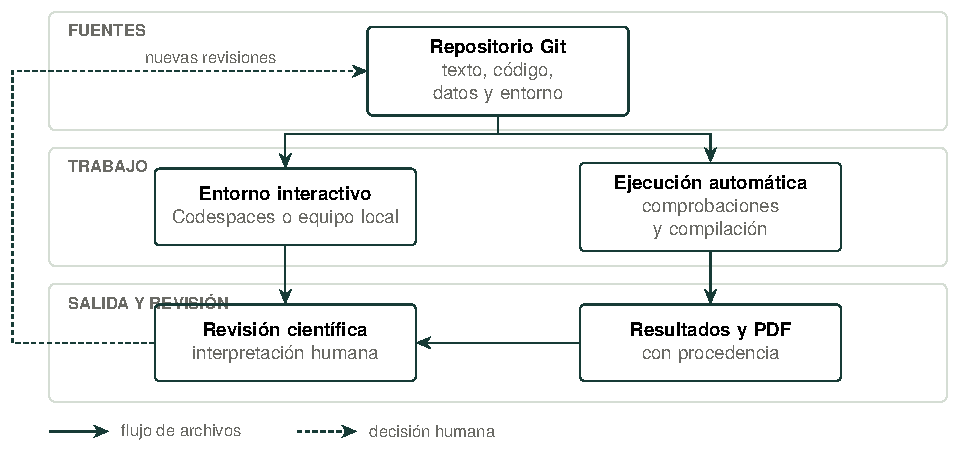
\includegraphics[width=160mm]{figures/modelo.pdf}
\caption{Arquitectura de referencia del trabajo docente y del demostrador editorial. El entorno interactivo y la ejecución automática consumen fuentes compartidas; la revisión científica sigue siendo una tarea humana.}\label{fig:arquitectura}
\end{figure}

\subsection{Una práctica de física que se pueda inspeccionar}
Como diseño docente proponemos partir de una distribución física sencilla producida a partir de datos abiertos. Una secuencia puede pedir reproducir la distribución de referencia, variar una selección, comparar el resultado y justificar la diferencia. Deben declararse unidades, muestra utilizada y normalización. Una comprobación automática puede detectar una columna ausente o una ejecución incompleta; no puede establecer por sí sola si una elección física es apropiada.

Conviene conservar una muestra pequeña para comprobar el funcionamiento y separar esa prueba del análisis completo. También debe evitarse que un cuaderno conserve resultados de una ejecución anterior incompatibles con su código actual. Ejecutarlo desde un estado limpio ayuda a detectar dependencias implícitas. Esta secuencia se propone como patrón de actividad; no se presenta como un nuevo resultado experimental ni se incluyen datos sintéticos que simulen una medición real.

\section{Resultados del análisis técnico}
\subsection{Opciones de despliegue y responsabilidades}
El cuadro~\ref{tab:plataformas} compara decisiones operativas. Binder 2.0 describe la publicación de entornos interactivos a partir de repositorios \cite{binderpaper}; el servicio público mybinder.org establece límites para sesiones efímeras \cite{binder}. JupyterHub permite administrar entornos por usuario y autenticación bajo control del operador \cite{jupyterhub}. Colab ofrece cuadernos gestionados con disponibilidad y límites variables \cite{colab}. Codespaces añade un entorno de desarrollo asociado al repositorio, con consumo de cómputo y almacenamiento facturable \cite{billing}.

\begin{table}[htbp]\centering\small
\caption{Comparación operativa según documentación de las plataformas consultada en octubre de 2026.}\label{tab:plataformas}
\begin{tabularx}{160mm}{@{}p{24mm}XXX@{}}\toprule
Opción & Administración & Conservación del trabajo & Condición a planificar \\
Codespaces & Servicio gestionado; configuración del repositorio & Espacio persistente hasta su eliminación; cambios a Git & Cuentas, cuotas, cómputo y almacenamiento \\
Binder público & Servicio comunitario; entorno desde repositorio & Sesión efímera; exportar cambios & Límites de sesión y capacidad compartida \\
JupyterHub & Operador institucional o proveedor & Depende del almacenamiento configurado & Autenticación, capacidad, respaldo y soporte \\
Colab & Cuadernos gestionados & Cuaderno guardado; estado de ejecución temporal & Límites variables y dependencias adicionales \\
\bottomrule\end{tabularx}
\end{table}


La comparación permite una decisión concreta: un ejercicio breve que solo necesita ejecutar un cuaderno tiene requisitos diferentes de un curso que enseña ramas, revisión de cambios y desarrollo de software. Codespaces encaja en este segundo objetivo si hay cuentas, conectividad y presupuesto; un JupyterHub institucional puede concentrar la administración cuando existe soporte local. Binder facilita demostraciones compartibles, mientras Colab ofrece una entrada rápida a cuadernos. La elección debe incluir el procedimiento para exportar el trabajo del alumno y conservarlo al terminar.

\subsection{Contexto docente e inventario de evidencia}
Los ejercicios públicos asociados a SILAFAE permiten examinar materiales de formación sin deducir de ellos tiempos de incorporación históricos. La 47.ª CERN School of Computing se celebró en Santiago del 11 al 24 de enero de 2026 \cite{csc}; su página de docentes incluye a Arturo Sánchez \cite{csclecturers}. Estos registros sitúan el contexto formativo. El cuadro~\ref{tab:evidencia} explicita qué evidencia sustenta cada afirmación del ensayo.

\begin{table}[tbp]
\caption{Evidencia de la trayectoria docente y alcance de cada registro.}\label{tab:evidencia}
\begin{tabularx}{\linewidth}{@{}>{\RaggedRight\arraybackslash}p{34mm}YY@{}}
\toprule
\cabecera{Registro} & \cabecera{Evidencia} & \cabecera{Alcance} \\
\midrule
\fila{SILAFAE, noviembre 2024} & Dos repositorios con SHA fechado & Contenido y recetas; no commit por alumno \\
\addlinespace
\fila{CSC, enero 2026} & Programa con responsables y horarios & Secuencia prevista; no tiempo real de preparación \\
\addlinespace
\fila{Selección CSC} & 70 plazas en diciembre; 69 seleccionados en enero & Cortes distintos; no asistencia a una sesión \\
\addlinespace
\fila{Ejercicios CSC} & SHA previo al curso y corrección del 12 de enero & Cambios en un ejercicio; no incidente operativo \\
\addlinespace
\fila{Evaluación por sesión} & Protocolo y plantillas de registro & Requiere consumo, incidencias y observaciones \\
\bottomrule
\end{tabularx}
\end{table}


El resultado técnico de esta lectura es separar tres objetos que suelen confundirse: un repositorio disponible, un entorno que ejecuta una tarea y una experiencia docente evaluada. Cada uno necesita una comprobación diferente. El repositorio permite inspección; una prueba limpia verifica ejecución; un registro por sesión permite estimar tiempos, incidencias y recursos. La arquitectura organiza esas comprobaciones sin sustituir una por otra.

\section{Protocolo de evaluación y gestión de recursos}
\subsection{Tiempo y costo}
La preparación del instructor y el inicio del estudiante deben medirse por separado. Para cada sesión se propone registrar un identificador anónimo, hora de inicio, primera ejecución válida, resultado de la comprobación y categoría de incidencia. El informe debe incluir participantes previstos, casos medidos, ejecuciones correctas y datos ausentes, junto con mediana y dispersión de los tiempos disponibles. Una preparación previa o una imagen precargada se declara como condición de la medición.

El registro económico distingue horas activas por tamaño de máquina, horas-núcleo, almacenamiento en GB-hora y uso de Actions para preconstrucciones. El almacenamiento sigue existiendo cuando el entorno está detenido; la tarifa y las cuotas aplicables se registran con su fecha \cite{billing}. El costo por participante requiere indicar si el denominador son inscritos, asistentes o personas que completaron la práctica. El repositorio adjunta plantillas vacías y un agregador que calcula consumos a partir de registros explícitos, sin asignar una tarifa universal ni reconstruir consumos históricos ausentes.

\subsection{Fallos que el diseño debe contemplar}
El cuadro~\ref{tab:riesgos} vincula riesgos operativos con señales y respuestas. Son escenarios de diseño, no incidentes atribuidos a una cohorte. Una prueba previa debe incluir cuenta de estudiante, permisos, arranque limpio y descarga de la muestra de datos. Con una alternativa local o un cuaderno exportable se puede continuar una parte de la actividad ante interrupciones del servicio.

\begin{table}[tbp]
\caption{Riesgos de diseño y respuesta propuesta. Son escenarios de diseño, no un registro de incidentes observados.}\label{tab:riesgos}
\begin{tabularx}{\linewidth}{@{}>{\RaggedRight\arraybackslash}p{34mm}YY@{}}
\toprule
\cabecera{Riesgo} & \cabecera{Señal a registrar} & \cabecera{Respuesta prevista} \\
\midrule
\fila{Acceso o permisos} & Inicio rechazado; categoría del error & Probar cuentas y acceso antes de clase \\
\addlinespace
\fila{Cuota o presupuesto} & Aprovisionamiento bloqueado & Revisar límites y responsable de facturación \\
\addlinespace
\fila{Conectividad} & Descarga incompleta o sesión interrumpida & Muestra reducida y materiales descargables \\
\addlinespace
\fila{Dependencia incompatible} & Validación fallida tras actualizar & Imagen identificada y prueba desde estado limpio \\
\addlinespace
\fila{Pérdida de trabajo} & Entorno eliminado sin exportación & Guardado en Git y copia de resultados \\
\bottomrule
\end{tabularx}
\end{table}


La evaluación del aprendizaje necesita una tarea adicional: interpretar una figura, justificar una selección o reproducir un análisis días después. El tiempo de aprovisionamiento mide acceso al entorno; la explicación del resultado mide otra dimensión. Un diseño comparativo debería mantener tarea y condiciones equivalentes y registrar experiencia previa, conectividad y apoyo recibido.

\section{El manuscrito como demostrador reproducible}
El repositorio que acompaña a este trabajo aplica el enfoque a la producción de los propios artículos. Cada manuscrito dispone de carpetas para texto, datos, fuentes, figuras y PDF. LaTeX reúne el contenido y las referencias; las figuras se generan como archivos vectoriales independientes. Un mismo comando realiza las comprobaciones y la compilación en el entorno de edición y en integración continua.

La configuración de GitHub Actions separa compilación y escritura. Las propuestas de cambio se compilan con permisos de lectura. En la rama predeterminada, un segundo trabajo recupera las salidas y actualiza los PDF mediante un commit. El token incorporado de GitHub evita que ese push dispare recursivamente otro flujo de push \cite{actions}. Una comprobación de revisión impide publicar un PDF generado a partir de fuentes anteriores a la cabeza actual de la rama. No se fuerza la escritura si la rama cambió.

Los nombres de los PDF son estables y cada nueva compilación sustituye los archivos visibles. Git conserva el historial, de modo que una única ruta actual no implica borrar versiones anteriores. Un manifiesto relaciona el PDF con hashes de sus fuentes y registra el motor de compilación. Este mecanismo facilita rastrear el producto editorial sin prometer identidad binaria entre versiones diferentes de TeX o paquetes.

El demostrador amplía un ejercicio previo para el Instituto de Ingeniería de Venezuela, cuyo repositorio separa datos, análisis, figuras e informes \cite{instituto}. Allí las automatizaciones entregan artifacts; aquí se añade la actualización controlada de los manuscritos en el repositorio. La diferencia responde al objetivo editorial de que un lector encuentre siempre el PDF actual. No se presenta la infraestructura de este paquete como un servicio ya desplegado en GitHub: requiere importar el repositorio y realizar su primera ejecución remota.

La verificación automática comprueba límites de los resúmenes, orden de referencias y errores de compilación. La revisión visual y científica continúa siendo necesaria. Un PDF actualizado puede contener una afirmación equivocada; la trazabilidad ayuda a localizarla y corregirla, pero no reemplaza la responsabilidad de los autores. La apertura pública del borrador debe acordarse con la política de la revista destinataria.

\section{Discusión}
La contribución de un entorno declarativo es hacer explícitas las dependencias y ofrecer un punto de partida compartido. En formación en física, ese punto de partida permite dedicar una secuencia docente a decisiones científicas: selección de datos, unidades, normalización e interpretación. Enseñar Git y automatización añade un registro de decisiones que puede revisarse con el estudiante y reutilizarse en otras disciplinas.

El servicio remoto redistribuye trabajo y costos. Parte de la instalación pasa al equipo docente; cuentas, cuotas y conectividad siguen condicionando la sesión. Una imagen fijada por digest identifica el software distribuido, pero datos externos y servicios requieren su propia conservación. El mantenimiento debe combinar una versión estable para cada curso con una ruta explícita de actualización y prueba.

\paragraph{Alcance y límites} El trabajo es un ensayo técnico basado en documentación y diseño de arquitectura. No dispone de registros individuales de incorporación, exportaciones de consumo ni evaluación causal del aprendizaje de las escuelas citadas. Por ello no informa cifras históricas de velocidad, costos o incidencia de fallos. La comparación de plataformas describe responsabilidades y condiciones documentadas, no un ensayo de rendimiento; las plantillas proponen cómo obtener esa evidencia en futuras sesiones.

\section{Conclusiones}
La computación transversal se concreta en prácticas que sobreviven al cambio de plataforma: describir dependencias, versionar procedimientos, ejecutar comprobaciones y conservar resultados interpretables. La comparación identifica dónde recae la administración y qué debe prever una actividad de física para compartir un entorno de trabajo.

La evaluación futura debe reunir tres tipos de evidencia: ejecución limpia del análisis, consumo y soporte de la sesión, y comprensión del estudiante. Mantenerlos separados permite mejorar la infraestructura sin confundir rapidez de acceso con aprendizaje. Las plantillas de registro y el ejemplo editorial ofrecen instrumentos concretos para iniciar esa evaluación.

\section*{Vínculos profesionales}
Arturo Sánchez Pineda mantiene una relación profesional con INAIT SA y participa en iniciativas de formación y ciencia abierta citadas en este trabajo. Las afiliaciones de este manuscrito son Creative Commons Venezuela y Creative Commons Switzerland. \editorialtodo{La declaración de financiación específica se completará antes del envío.}


\begin{thebibliography}{99}\small\setlength{\itemsep}{2pt}\setlength{\parskip}{0pt}
\bibitem{wilson} Wilson G, Bryan J, Cranston K, Kitzes J, Nederbragt L, Teal TK. Good enough practices in scientific computing. PLoS Comput Biol 13(6), e1005510 (2017). \url{https://doi.org/10.1371/journal.pcbi.1005510}.

\bibitem{transversal} Sánchez Pineda A. A proposal for Transversal Computer-related Strategies \& Services for Scientific and Training efforts for the LASF4RI. arXiv:2104.09622 (2021). \url{https://doi.org/10.48550/arXiv.2104.09622}.

\bibitem{whitepaper} Sánchez Pineda A. An empirical case and ongoing efforts on Transversal Computer Strategies \& Services for Scientific and Training efforts for the LASF4RI. Zenodo, v3 (2024). \url{https://doi.org/10.5281/zenodo.13324266}.

\bibitem{abstract} Sánchez Pineda A. Automated, reproducible cloud workspaces for HEP training in Latin America with cloud-based Git Codespaces and CI. Resumen 667, ICHEP 2026. Captura de Indico del 14 de marzo de 2026, proporcionada por el autor. \url{https://indico.cern.ch/event/1522800/abstracts/201558/}.

\bibitem{atlas} Sánchez Pineda A. Boosting high-energy physics education around the world with ATLAS Open Data. ATLAS/CERN (2018). \url{https://atlas.cern/updates/blog/HEP-education-worldwide-with-atlas-open-data}.

\bibitem{contexto} Sánchez Pineda A. De los datos abiertos al conocimiento compartido: fuentes y antecedentes CHEP. Repositorio de la presentación para el Instituto de Ingeniería, SOURCES.md (2026). \url{https://github.com/artfisica/presentacion-Instituto-de-Ingenieria-Venezuela}.

\bibitem{chep} Sánchez Pineda A, Guerrieri G. A proposal for Open Access data and tools multi-user deployment using ATLAS Open Data for Education. EPJ Web Conf 251, 01008 (2021). \url{https://doi.org/10.1051/epjconf/202125101008}.

\bibitem{devcontainers} GitHub. Introduction to dev containers. Documentación técnica, consulta: 21 de octubre de 2026. \url{https://docs.github.com/en/codespaces/setting-up-your-project-for-codespaces/adding-a-dev-container-configuration/introduction-to-dev-containers}.

\bibitem{repos} LAA-HECAP. Repositorios docentes jupyter-on-codespaces y exercises-silafae. Consulta: 21 de octubre de 2026. \url{https://github.com/laa-hecap/jupyter-on-codespaces}; \url{https://github.com/laa-hecap/exercises-silafae}.

\bibitem{csc} CERN. 47th CERN School of Computing -- Latin America 2026, 11--24 de enero de 2026. Programa y materiales. \url{https://indico.cern.ch/event/1551289/timetable/?view=standard_numbered}.

\bibitem{actions} GitHub. Triggering a workflow. Documentación técnica, consulta: 21 de octubre de 2026. \url{https://docs.github.com/en/actions/how-tos/write-workflows/choose-when-workflows-run/trigger-a-workflow}.

\bibitem{instituto} Sánchez Pineda A. De los datos abiertos al conocimiento compartido. Materiales docentes y ejercicios de automatización (2026). \url{https://github.com/artfisica/presentacion-Instituto-de-Ingenieria-Venezuela}.
\end{thebibliography}

\end{document}
